% !TEX root = ../main.tex

\chapter{Introduction}
\label{ch:introduction}
Machine learning, particularly deep learning using neural networks, has greatly benefitted from the availability of large amounts of data. Neural networks have demonstrated significant potential in solving a wide range of tasks. By examining the potential of binary trees, this thesis aims to provide insights into alternative models that could complement or even surpass the performance of traditional neural networks in certain reinforcement learning scenarios.

\section{Neural Networks}

Neural networks are a type of machine learning that takes inspiration from the structure and function of neurons in the human brain. The model is composed of layers of interconnected artificial neurons, which process and transmit information. In neural networks, the input data is first passed through the first layer, and then each subsequent layer receives the output from the previous layer as input.

Neural networks learn by adjusting the connections, or weights, between neurons based on the input data and the desired output. The output of a single neuron is calculated by combining the inputs from the previous layer with the corresponding weights, and adding a bias term if applicable. This weighted sum is then passed through an activation function, which transforms the sum into the output of the neuron. Common activation functions include the sigmoid function, hyperbolic tangent (tanh), and rectified linear unit (ReLU). The choice of activation function depends on the specific task and the architecture of the network.

A neural network can be represented as a computational graph that combines a series of simple functions to produce complex and high-dimensional representations, which capture the underlying function that enables the network to make accurate predictions. This ability to learn multiple levels of abstraction through function composition is one of the key strengths of neural networks and sets them apart from traditional linear models. Figure \ref{fig:neural_network} illustrate a human-readable way to represent neural networks.

\begin{figure}[!ht]
\centering
\fbox{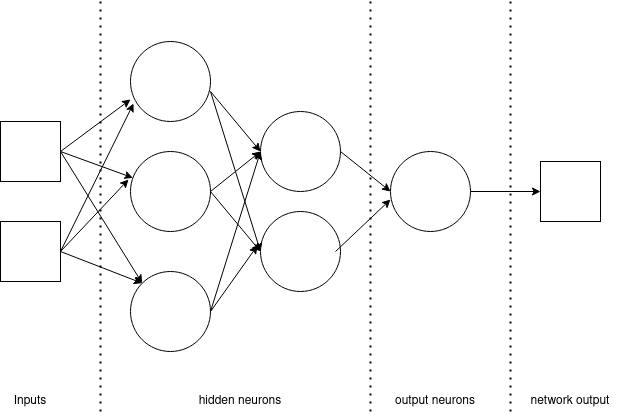
\includegraphics[width=.8\textwidth]{neural_network}}
\caption[Neural network and its components]{
  \textbf{Neural network} process incoming input data through a structure consisting of two hidden layers, one with three neurons and one with two, and an output layer with a single neuron. The output produced by the network is determined by passing it through an activation function, which represents the final output of the network.
  }
\label{fig:neural_network}
\end{figure}


The most widely used optimization algorithm for the learning process is gradient descent, which helps find the optimal weights by minimizing the error between the network's predictions and the actual output. Backpropagation is a powerful tool for efficiently calculating the gradient of the loss function with respect to the weights. This is done through a forward pass, where the predicted outputs and intermediate node values are determined, followed by a backward pass, where the gradient of the loss function with respect to each weight is calculated using the chain rule of calculus. The gradient is then used to update the weights through gradient descent until the weights converge to values that minimize the loss function. For backpropagation to be effective, the activation functions of the artificial neurons must be continuous and easily differentiable (\cite{goodfellow_deep_2016}).

The structure of a neural network, including the number of layers and number of neurons per layer, significantly impacts its ability to solve tasks. A larger number of layers allows for the approximation of more complex functions, but can also result in overfitting, where the model performs well on training data but poorly on new data. The field dedicated to finding optimal structures is referred to as neural architecture search.

\section{Binary trees}

Trees are a type of data structure that are commonly used in computer science and mathematics. They consist of nodes, which are connected by edges. Trees are special because they are a type of graph that is undirected, connected, and acyclic, meaning that nodes are connected by edges, but there are no loops or cycles in the graph.

In a tree, each node is either a parent or a child. The top node, with no parent, is called the root, while the bottom nodes with no children are called leaves. The distance from the root node determines the level of the node, with the root at level 0 and its children at level 1, and so on. Nodes on the same level are called siblings.

Binary trees are a specific type of tree in which every node, except for leaves, has at most two children, which are called the left and right nodes. Binary trees are easy to understand and visualize, making them useful for a variety of applications. An example of a binary tree is shown in Figure \ref{fig:binary_tree}.

In addition to binary trees, there are other types of trees that are commonly used in computer science and data structures. One example is the "n-ary" tree, which allows nodes to have any number of children. Another example is the "balanced" tree, which is designed to keep the tree's height as small as possible, while still allowing for efficient searches and insertions. Balanced trees come in several different varieties, such as red-black trees and B-trees, each with their own specific balancing algorithms and performance characteristics (\cite{goodrich_data_nodate}).

For this project, a specific type of binary tree will be used, in which all nodes except the leaves have exactly two children, rather than at most two children like in classical binary trees.

\begin{figure}[!ht]
\centering
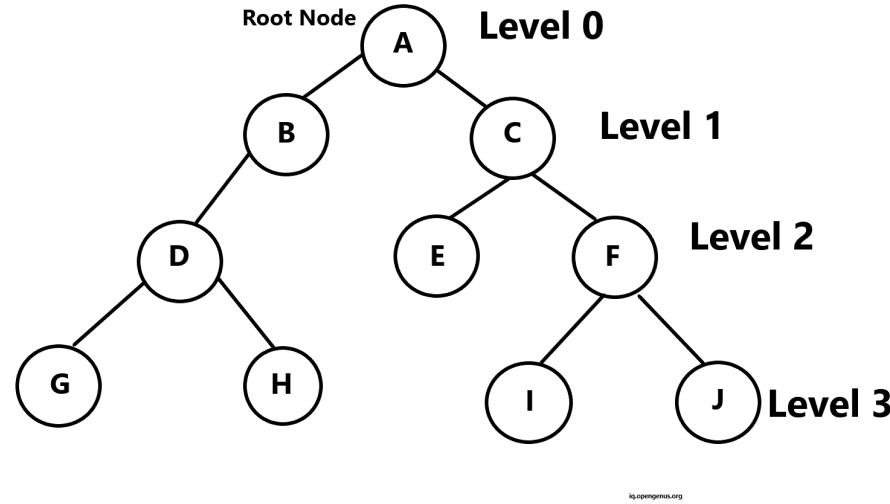
\includegraphics[width=.5\textwidth]{binary_tree}
\caption[Binary tree]{
  \textbf{Binary tree} where the blue nodes illustrate leafs and the red node is the root of the tree
  }
\label{fig:binary_tree}
\end{figure}

Binary trees offer several advantages over other data structures. One of the main advantages is their ability to efficiently search, insert, and delete elements. Another advantage is their simplicity and interpretability, as the structure of a binary tree is easy to understand and visualize. This makes it easier to understand how decisions are made and identify errors in the model. In the context of reinforcement learning, binary trees can provide better approximation of discontinuities by allowing for different actions depending on the chosen path. This will be one of the motivations of the project discussed later.

\section{Architecture search}

Neural networks have seen significant advancements in recent years, due in large part to the availability of vast amounts of data. Deep neural networks have demonstrated their ability to solve a wide range of problems, such as image recognition and translation. However, finding the optimal number of layers and nodes, referred to as the architecture, for a neural network to efficiently solve a problem is still a challenging task. One approach is to try different architectures and evaluate their performance, which can be time and effort consuming when dealing with deep, complex neural networks as the structure needs to be designed by hand. Another approach is to use neural architecture search (NAS), which automates the process of finding an appropriate architecture for a specific task. Researchers continue to investigate effective methods for architecture search, with evolutionary algorithms, reinforcement learning, gradient-based optimization, or a combination of these techniques, being commonly used to explore the space of possible architectures(\cite{elsken_neural_nodate}).

Until now, neural architecture search algorithms tend to be slow and expensive due to the need to train a large number of candidate networks to inform the search process. The paper by \cite{mellor_neural_nodate} showed that a possible solution to speed up this process would be to perform neural architecture search without any network training. The authors implemented a search algorithm called "NASWOT," which only makes observations on the initial untrained networks in the scope of convolutional networks.

The concept of automatically searching for structures that improve model performance without manual intervention can also be applied to binary tree models. A complex reinforcement learning task would usually require a larger binary tree, as this would increase the search space for policies and, thereby, improve the probability of finding good solutions. To achieve this, it is important to adapt the size of the tree according to the complexity of the task. By dynamically incrementing the size of the tree, various strategies can be implemented. The first decision is where to add or remove new nodes in the tree and how many to add. For example, nodes could be added from left to right until the level is full and then proceed to the next layer, or they could be added to a randomly selected leaf, as is the case in this project. Another decision is when to change the size of the tree dynamically. If the tree structure changes too rapidly, the algorithm may not have enough time to search for solutions in the actual search space, whereas waiting too long could result in the algorithm getting stuck in a local optimum and wasting time. Therefore, it is important to strike a balance and change the size of the tree at the right moment. Additionally, it is important to decide which functions the newly created nodes should have. Should they be the same as their parent nodes, or should they be different? Finally, another surprising consideration is whether the newly added nodes should be leaves, which is not the case in this project, as you will see later.

All of these decisions and more must be made and possibly compared when deciding which node-adding strategy to implement. It is important that, even if the tree structure changes, the mathematical equation of the tree remains invariant, which can be a challenging aspect to implement and can also limit the strategies that can be used.


\section{Motivation and Hypothesis for Discontinuous Models in Reinforcement Learning}

In the context of this project, the observation is that current models are typically continuous, but many control tasks are not. Neural networks for example need continuous functions in backpropagation. The basic idea behind backpropagation is to adjust the weights of the network by calculating the gradient of the loss function with respect to the weights. This is done by propagating the error backwards through the network, hence the name "backpropagation". The goal is to minimize the error of the network, the next time it makes a prediction and it is repeated for many iterations until the model converges to a set of weights that minimize the error.
An example of a non-continuous problem this is swing up cartpole. This task consists of a pendulum fixed to a cart with a fixed joint above and a loose joint below, which is swung up in a first step and then stabilized in the second step.Figure\ref{fig:swing_up} illustrates this problem. When attempting to approximate the function that models this task, it becomes apparent that the function will have a discontuinity. Due to the two distinct tasks involved, the agent must be able to recognize when the first task is complete and the second one begins. In the real world, there are many control problems that are not continuous.
The hypothesis is that discontinuous models would have an advantage in addressing these tasks. Binary trees should allow for the approximation of discontinuities. This is achieved by using a hyperplane to partition the observation space, and depending on the chosen subtree (by going to the left or right child), a different policy will be used. To test this hypothesis, multiple individuals can be evaluated in the environment (by running them through the fitness function) and their performance analyzed, along with other metrics such as the number of individuals that successfully solve the task. Hyperparameters also play an important role in improving the performance of individuals in the environment.

\begin{figure}[!ht]
\centering
\fbox{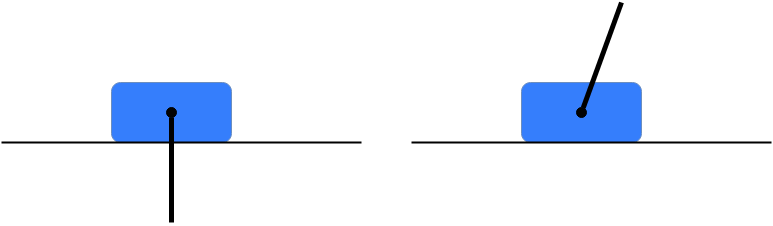
\includegraphics[width=.8\textwidth]{swing_up}}
\caption[Non-continuous control task]{
  \textbf{Cart-pole swing up problem} On the left side, the initial state of the problem is depicted where the pole is pointing downwards and needs to be swung up by moving the blue cart on the horizontal line. On the right side, the cart has successfully managed to swing the pole up and now needs to stabilize it vertically.
  }
\label{fig:swing_up}
\end{figure}

\section{Contribution}

This thesis builds on the prior work "Alternative Models for Direct Policy Search in Reinforcement Learning Control Problems" (\cite{masanti_alternative_nodate}), which recognizes the potential of using binary trees to address reinforcement learning challenges. The main contribution of this thesis is to enhance the efficiency of the previous model by introducing a novel function that dynamically increases the size of the binary tree. This new function represents a crucial step towards enabling architecture search for binary trees and has the potential to significantly improve their performance in solving reinforcement learning tasks. It is important to note, however, that only one possible tree-growing strategy will be tested, and no comparison of different structures will be made. The goal is solely to increase the tree size until the given task can be solved.

The thesis included a code structure for binary tree models, serving as a basic starting point. The first step was to make the code work. Once the binary tree model was functional, a basic architecture search technique was implemented, and its effectiveness was evaluated on several reinforcement learning problems.
